\documentclass[a4paper]{article}

\usepackage[utf8]{inputenc}
\usepackage[english]{babel}
\usepackage[margin=2.54cm]{geometry}
\usepackage{siunitx} % voor m/s, graden Celsius
\usepackage{parskip} % geen tab na paragraafeinde
\usepackage{amsmath, amssymb} % voor equation*
\usepackage[version=4]{mhchem} % chemie
\usepackage{graphicx} % afbeeldingen
\usepackage{fancyhdr} % headers en footers
\usepackage{xcolor} % kleuren
\usepackage[bookmarksnumbered]{hyperref} % links naar tabellen en figuren
\usepackage[normalem]{ulem}

\hypersetup{
  colorlinks   = true, %Colours links instead of ugly boxes
  linkcolor    = blue, %Colour of internal links  
  citecolor    = blue, %Colour of internal links
}

\newcommand{\Ums}{[\si[per-mode=symbol]{\meter\per\second}]}
\newcommand{\Um}{[\si{\meter}]}

\title{Principles of Groundwater Flow}
\author{Tim Weijers \and Vincent Kuhlmann}
\date{\today}

\begin{document}
\maketitle

{
\hypersetup{linkcolor=black}
\tableofcontents
}
\newpage

\section{The polder problem}
\begin{enumerate}

\item
We consider a \underline{vertical cross section} of an \textsc{infinitely long polder}. The polder consists of a confined aquifer with hydraulic conductivity $k_1$ \Ums{} and thickness $D$ \Um. The \textbf{top} layer has thickness $b$ \Um{} and hydraulic conductivity $k_2$ \Ums. We refer to $h_p$ \Um{} as `Polder level'. Note that $h(+\infty) = h_p$. The ambient air temperature is \SI{23}{\celsius}.

The hydraulic head distribution in the Polder satisfies the general solution of the well-known \emph{Polder Problem}\cite{alfonso2010}:
\begin{equation} \label{eq:polder}
h(x) = C_1e^{+\frac{x}{\lambda}} + C_2e^{-\frac{x}{\lambda}} + h_p
\end{equation}
Where $\lambda$ is the seepage factor
\begin{equation}
\lambda = \sqrt{\frac{k_1}{k_2}bD}
\end{equation}
and $C_1$ and $C_2$ are yet unknown constants.

\begin{enumerate}

\item Determine the constants $C_1$ and $C_2$
\item Explain in words why it follows from \autoref{eq:polder}, that the following equalities must both hold:
\begin{align*}
Q'(0) &= \frac{k_1D}{\lambda}(h_0 - h_p)\\[1em]
Q'(0) &= \int_0^{+\infty}q_z(s)ds
\end{align*}

\end{enumerate}

\item
Balance the following redox equation (using \ce{H+} and \ce{H3O-})
\begin{equation*}
\ce{MnO2(s) + S2O3^2- -> MnOOH(s) + SO3^2-}
\end{equation*}

\end{enumerate}

\section{Mineral compositions}
\autoref{table:mineral} contains information about the composition of certain minerals.

\begin{table}[h!]
\centering
\begin{tabular}{|r|c|c|}
\hline
\textbf{Mineral} & Albite & Anorthite \\
\hline
\ce{SiO2} & 68.74 & 43.19\\
\hline
\ce{Na2O} & 11.82 & 0.0 \\
\hline 
\end{tabular}
\caption{Mineral compositions in oxide wt. \%}
\label{table:mineral}
\end{table}

\section{Kaolinite in cuprite}
\subsection{Chemical composition}
Kaolinite is a {\LARGE clay mineral}, with the chemical composition \ce{Al2Si2O5(OH)4}. Cuprite is a \textcolor{brown}{brownish}-\textcolor{red}{red} mineral. The average kaolin price is estimated to reach \sout{\$160} \$180 per ton by 2025.
\subsection{Deposits in Nevada}
Recent measurements show deposits of the mineral kaolinite in cuprite in the Nevada desert, as seen in \autoref{fig:nevadasam}.
\begin{figure}[h]
\centering
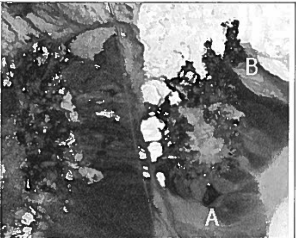
\includegraphics[width=0.5\textwidth]{kaolinite}
\caption{SAM result for Kaolinite in Cuprite, Nevada desert in the USA deribed on an AVIRIS image.}
\label{fig:nevadasam}
\end{figure}

\bibliographystyle{plain}
\bibliography{literatuur.bib}

\end{document}
